\section{HILS Communication Mechanism Library Implementation}

The library is implemented using object-oriented programming paradigm. Some
classes are exposed by the library to allow the use of APIs for communication in
the HILS system. These classes abstracts the process of data serialization,
deserialization, sending, and receiving so the library user only need to call a
class method to get usable data.

A ``conceptual package diagram'' that shows classes exposed by the library can
be seen in Fig.~\ref{fig-section-5-conceptual-package-diagram}. The consumer
component of the library exposes a class called \texttt{Car\-la\-Ser\-vice} and
producer component exposes four classes called \texttt{G\-n\-s\-s\-Hand\-ler},
\texttt{Li\-dar\-Hand\-ler}, \texttt{Ca\-me\-ra\-Hand\-ler}, and
\texttt{Con\-trol\-Hand\-ler}. Do note, the interfaces \texttt{SensorReader} and
\texttt{\{Gnss,Lidar,Camera,Control\}Processor} are not implemented and are only
in the diagram for easier understanding.

On the other hand, the \texttt{Endpoint} interface is real and it is for
abstracting the sending and receiving process in the library. Said interface is
made abstract so adding and changing communication protocol/method can be easily
done. For now, the interface is only implemented by the classes
\texttt{ZeroMQEndpoint} and \texttt{ZeroMqSocket}.

\begin{figure}[htbp]
	\centerline{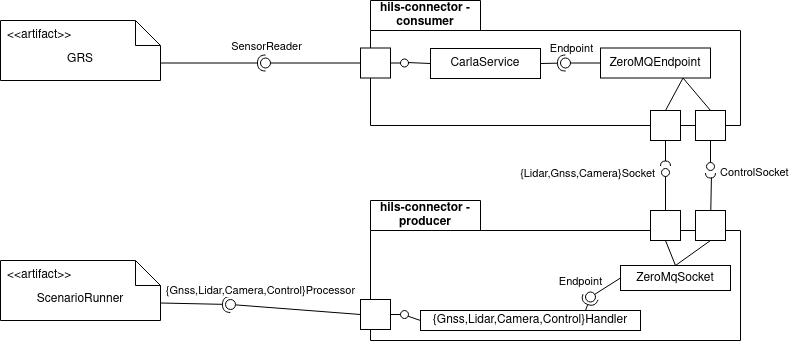
\includegraphics[width=0.45\textwidth]{resources/chapter-4/conceptual-package-diagram.png}}
	\caption{Conceptual Package Diagram}
	\label{fig-section-5-conceptual-package-diagram}
\end{figure}

The complete class diagram for the consument component can be seen in the
Fig.~\ref{fig-section-5-consumer-class-diagram}. While the complete producer class
diagram can be seen in the Fig.~\ref{fig-section-5-producer-class-diagram}.

\begin{figure}[htbp]
	\centerline{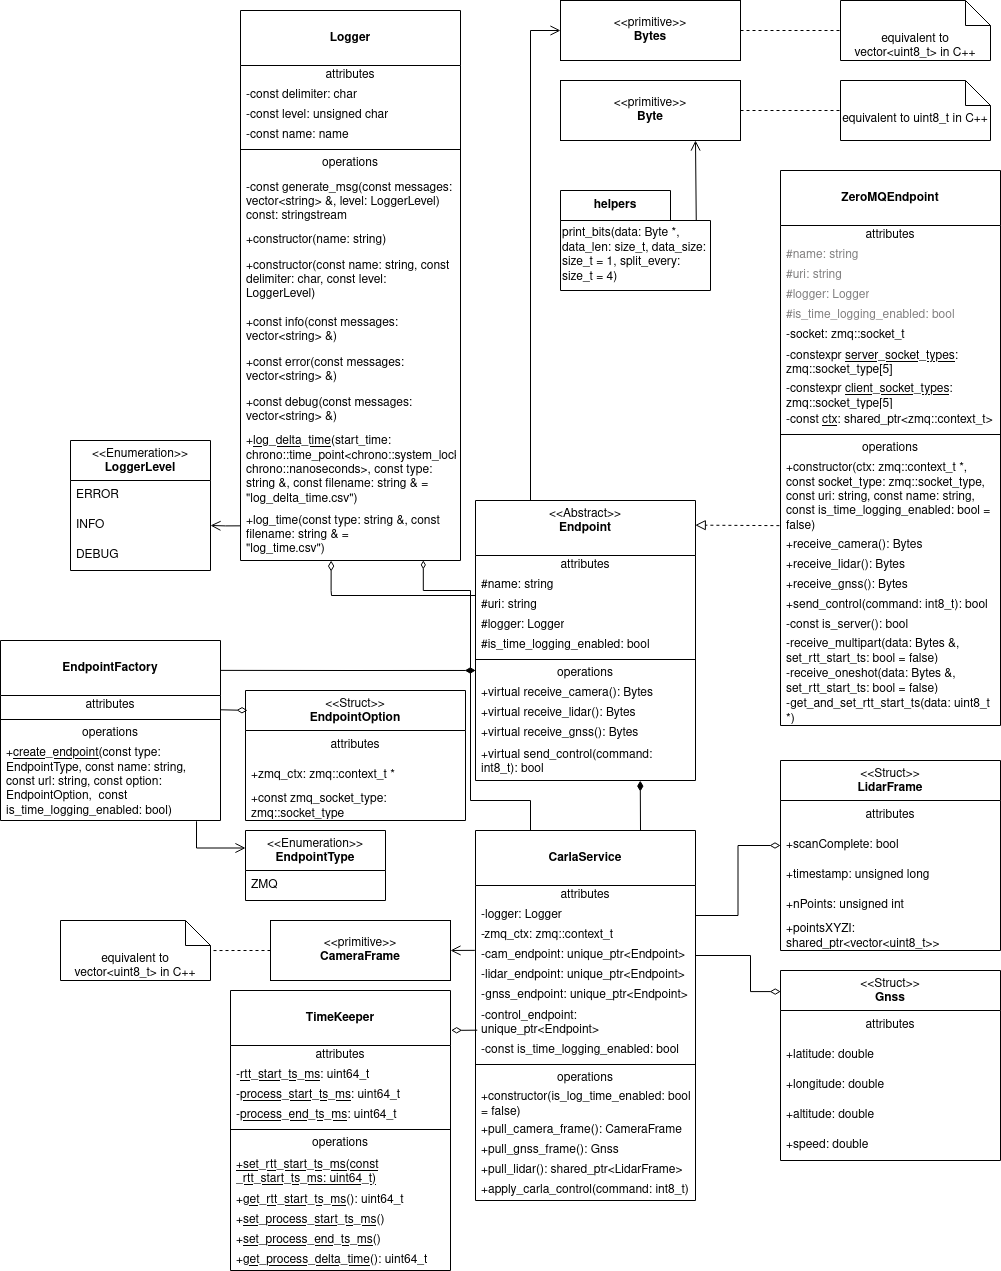
\includegraphics[width=0.45\textwidth]{resources/chapter-4/consumer-class_diagram.png}}
	\caption{Consumer Class Diagram}
	\label{fig-section-5-consumer-class-diagram}
\end{figure}

\begin{figure}[htbp]
	\centerline{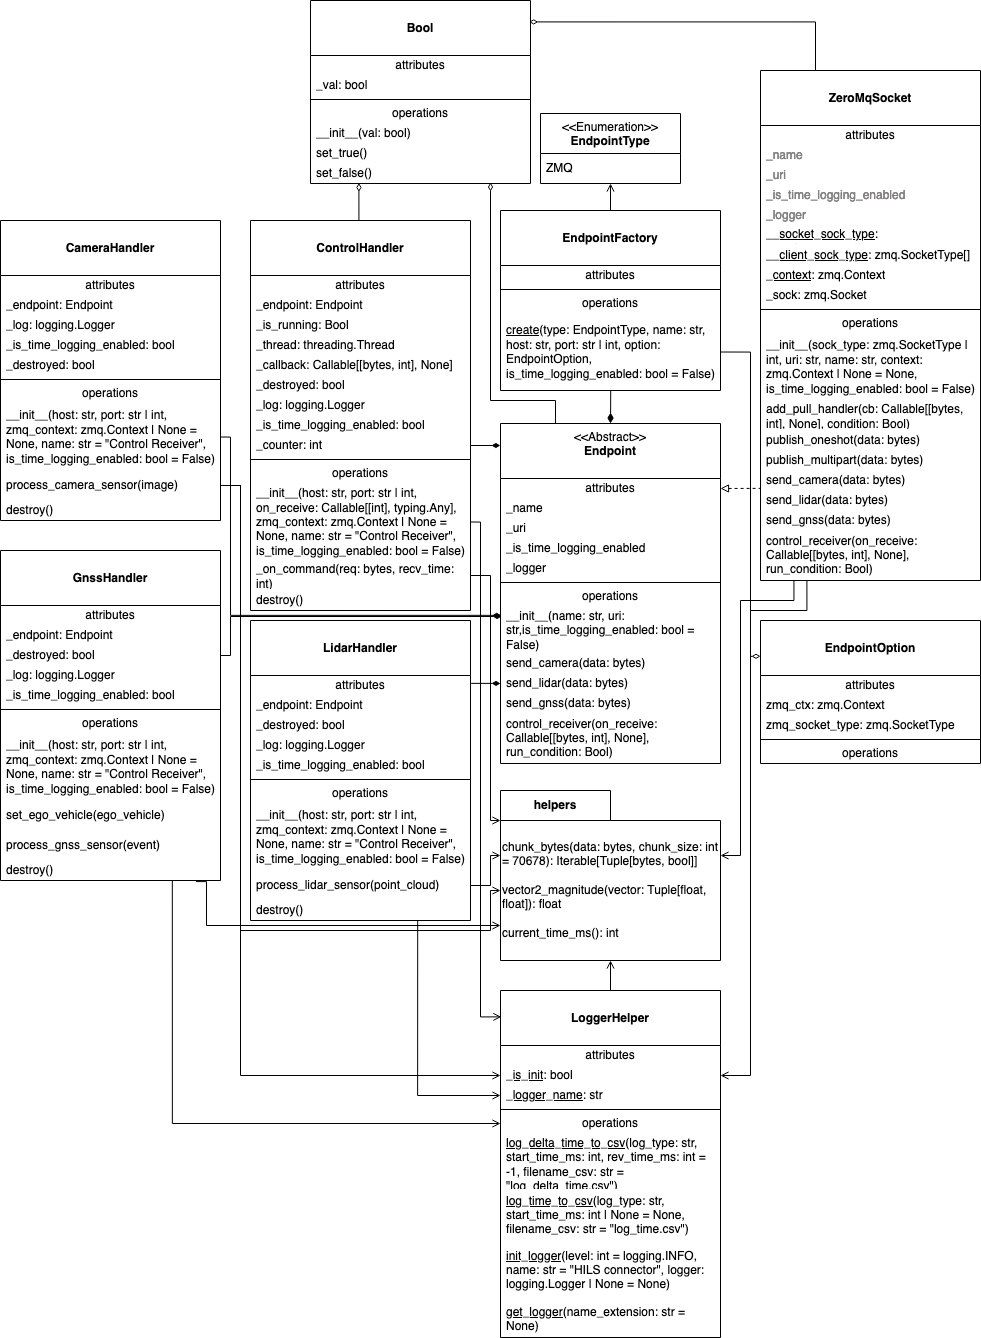
\includegraphics[width=0.45\textwidth]{resources/chapter-4/producer-class_diagram.png}}
	\caption{Producer Class Diagram}
	\label{fig-section-5-producer-class-diagram}
\end{figure}